\section{Usage} % (fold)
\label{sec:usage}
This section displays how to use the quiz system for it's intended purpose. The different parts of the system have been split up into different subsections for convenience.

\subsection{Creating a New Quiz} % (fold)
\label{sub:creating_a_quiz}
Creating a new quiz is a very simple process. Select your house and year from the drop down lists on the menu, and then press the ``Create a new quiz'' button.
\begin{figure}[h!]
  \centering
  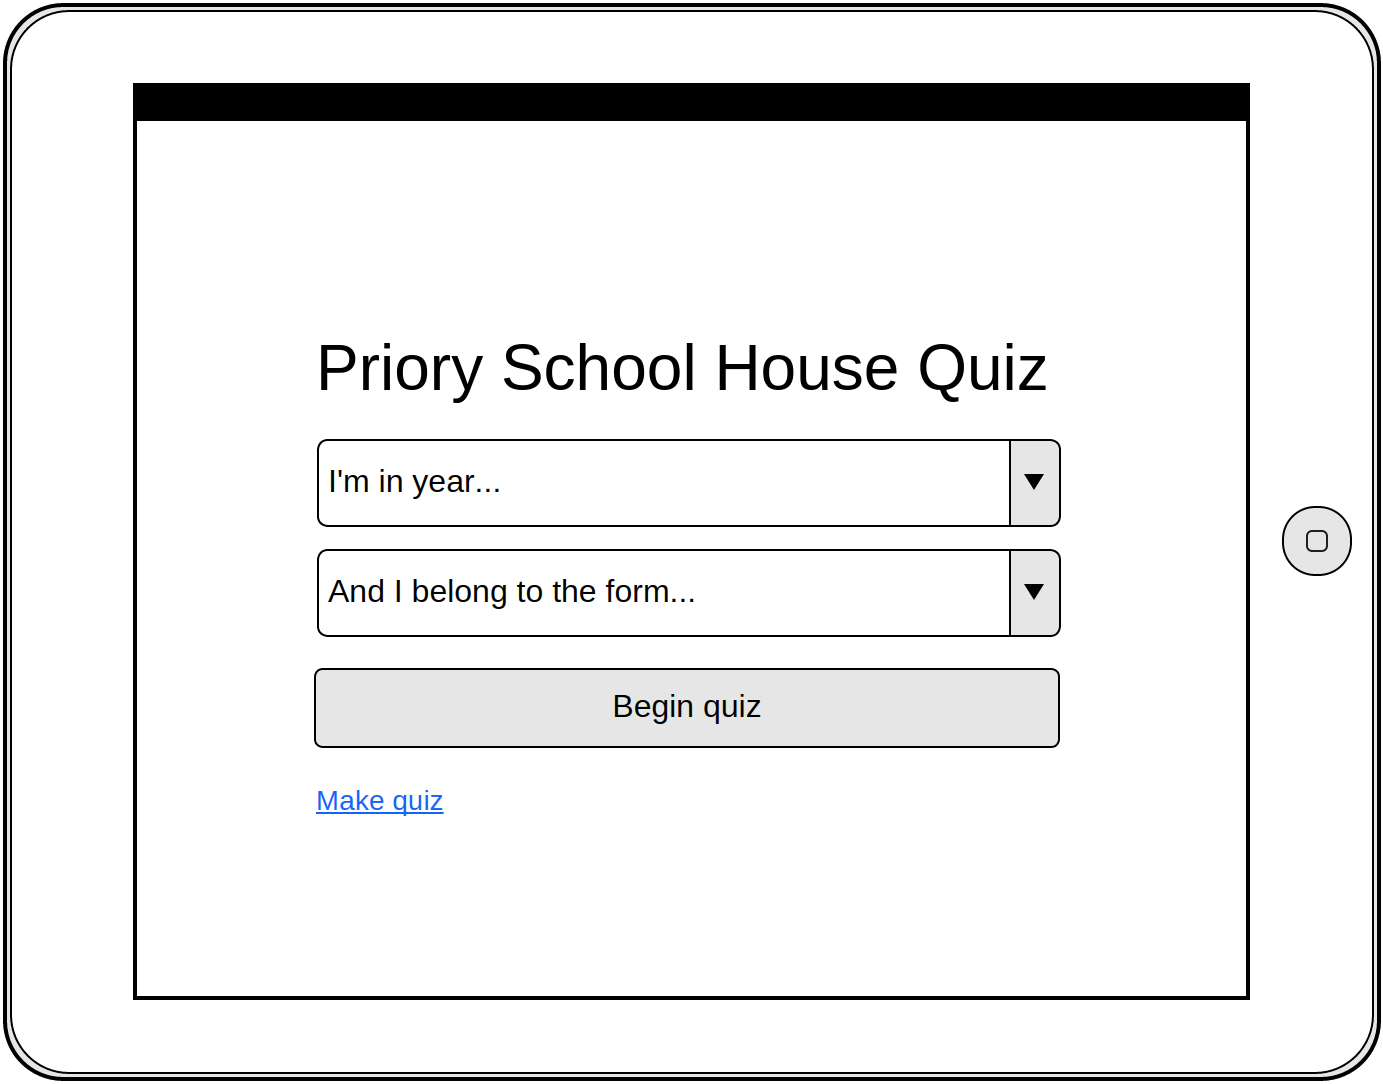
\includegraphics[scale=0.35]{user_guide/usage/login}
  \caption{The main login screen, where you can select your house and year and create a new quiz.}
\end{figure}
% subsection creating_a_quiz (end)

\clearpage

\subsection{Editing a Quiz} % (fold)
\label{sub:editing_a_quiz}
The interface for adding questions and answers to a quiz is similar to other quiz creation systems you may have used in the past. When a quiz is first created, there is one question, with four answers - all of these can be edited.

\subsubsection{Editing a Question} % (fold)
\label{ssub:editing_a_question}
To edit a question's title, simply click or tap the current title, and type in your changes. Tap out again once you've finished.
\begin{figure}[h!]
  \centering
  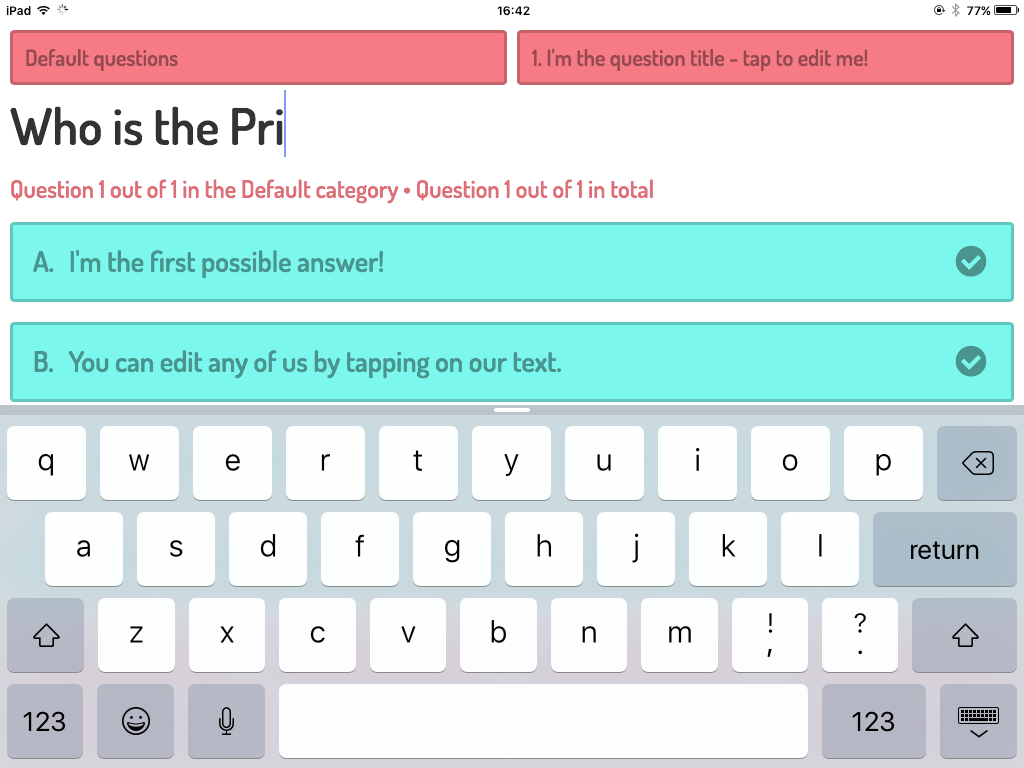
\includegraphics[scale=0.25]{user_guide/usage/edit_question}
  \caption{Typing a new question name.}
\end{figure}
% subsubsection editing_a_question (end)

\clearpage

\subsubsection{Editing an Answer} % (fold)
\label{ssub:editing_an_answer}
To edit a question's answer, simply click or tap the current answer, and type in your changes.
\begin{figure}[h!]
  \centering
  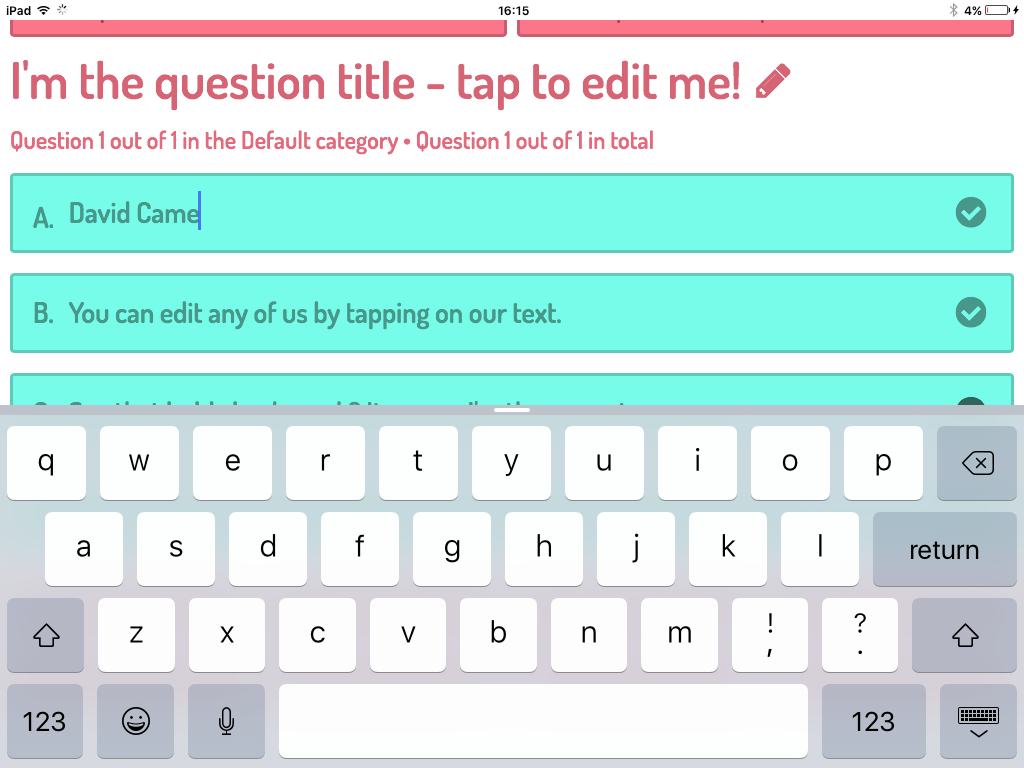
\includegraphics[scale=0.25]{user_guide/usage/edit_answer}
  \caption{Typing a new answer body.}
\end{figure}
% subsubsection editing_an_answer (end)

\subsubsection{Marking an Answer as Correct} % (fold)
\label{ssub:marking_an_answer_as_correct}
To mark an answer as correct, tap the tick icon at the end of the answer, shown with a red circle. The answer currently marked as correct will no longer be so.
\begin{figure}[h!]
  \centering
  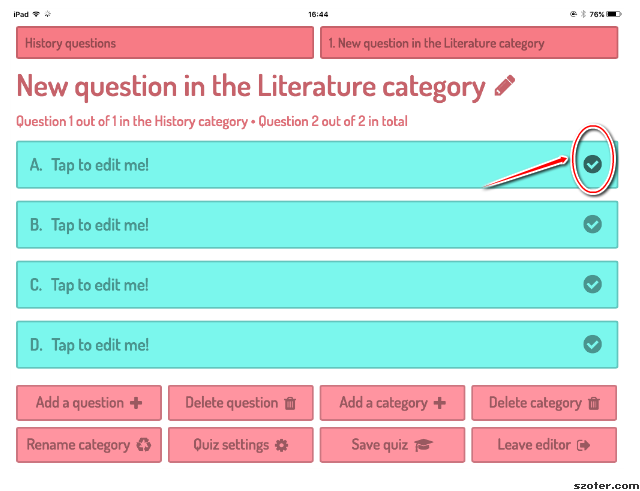
\includegraphics[scale=0.25]{user_guide/usage/change_answer}
  \caption{Tap on a tick to mark that answer as correct.}
\end{figure}
% subsubsection marking_an_answer_as_correct (end)

\subsubsection{Adding a Question} % (fold)
\label{ssub:adding_a_question}
To add a new question, simply press the ``Add Question'' button.
% subsubsection adding_a_question (end)

% subsection editing_a_quiz (end)

\subsection{Scheduling a Quiz} % (fold)
\label{sub:scheduling_a_quiz}
To schedule a quiz, perform the following steps:

\begin{enumerate}
\item Tap the ``Quiz settings'' button.
\item Enter the date and time you wish the quiz to begin.
\item Tap the ``Save settings'' button to exit the settings panel.
\item Tap the ``Save quiz'' button.
\end{enumerate}

Your quiz has now been scheduled, and will take place at the set time.
\begin{figure}[h!]
  \centering
  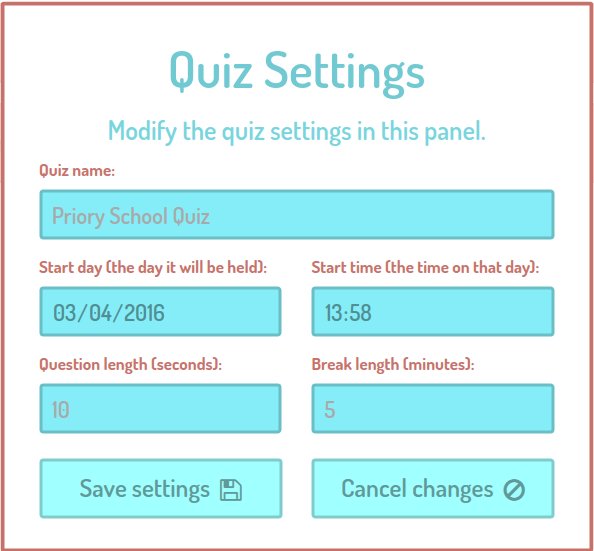
\includegraphics[scale=0.25]{user_guide/usage/schedule}
  \caption{Scheduling a quiz.}
\end{figure}

When students join the quiz at least 20 minutes before the time you have scheduled, they will be met with a countdown showing how long is left before the quiz begins. This will automatically change, and will begin the quiz once the time has elapsed.

\begin{figure}[h!]
  \centering
  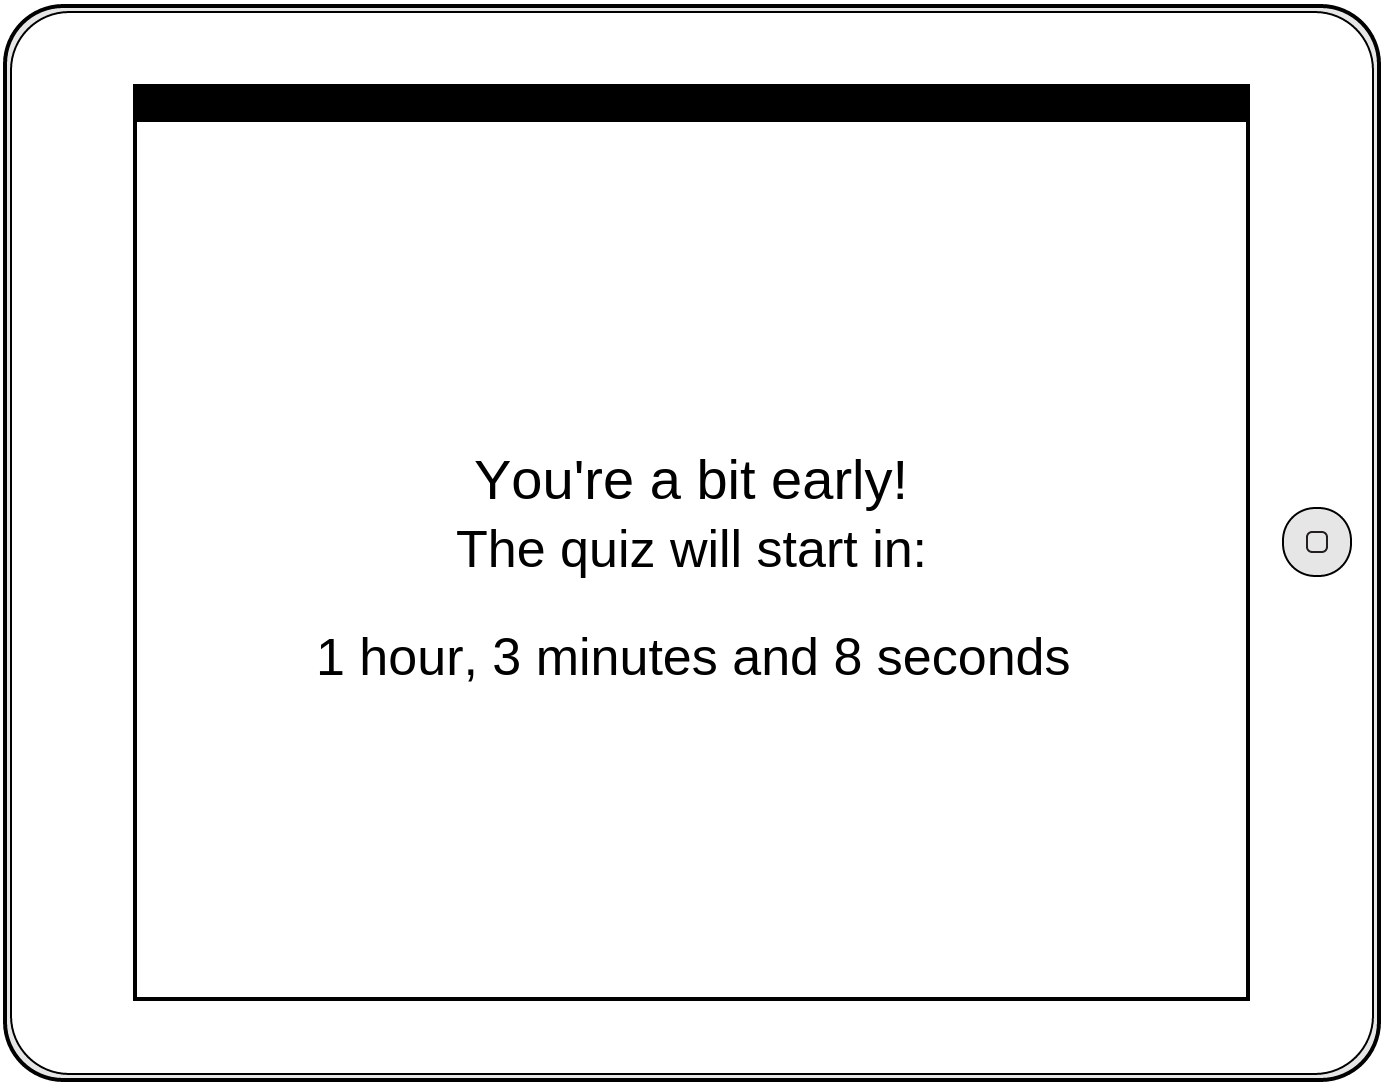
\includegraphics[scale=0.35]{user_guide/usage/countdown}
  \caption{The countdown displayed when students are early.}
\end{figure}
% subsection scheduling_a_quiz (end)

\subsection{Loading a Quiz} % (fold)
\label{sub:loading_a_quiz}
If you wish to load a quiz that has been created earlier, for further editing, press the ``Load quiz'' button on the main menu, and locate the quiz you wish to edit by its title and schedule date. From there, press the ``Edit quiz'' button, and you will be taken to the familiar quiz editing interface. If you are online, or there are no quizzes, the box will alert you to this, as shown in the figures.

\begin{figure}[!htbp]
\centering
\begin{subfigure}{0.5\textwidth}
  \centering
  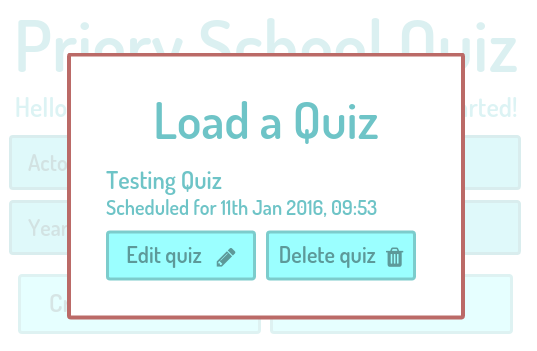
\includegraphics[width=0.95\linewidth]{testing/load_quiz/single_quiz}
  \caption{Five quizzes (extreme)}
  \label{fig:sub2}
\end{subfigure}
\label{fig:test}
\end{figure}
\begin{figure}[!htbp]
\centering
\begin{subfigure}{0.5\textwidth}
  \centering
  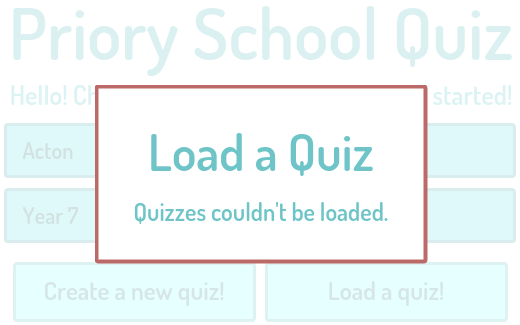
\includegraphics[width=0.95\linewidth]{testing/load_quiz/offline}
  \setcounter{subfigure}{2}%
  \caption{No connection (erroneous)}
  \label{fig:sub1}
\end{subfigure}%
\begin{subfigure}{0.5\textwidth}
  \centering
  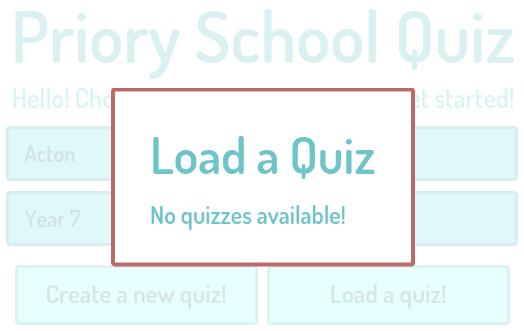
\includegraphics[width=0.95\linewidth]{testing/load_quiz/no_quizzes}
  \setcounter{subfigure}{3}%
  \caption{No quizzes (null)}
  \label{fig:sub2}
\end{subfigure}
\caption{The load quiz dialog.}
\label{fig:test}
\end{figure}
% subsection loading_a_quiz (end)

\subsection{Deleting a Quiz} % (fold)
\label{sub:deleting_a_quiz}
Deleting a quiz is also very simple. Press the ``Load quiz'' button on the main menu, and locate the quiz you wish to edit by its title and schedule date. From there, press the ``Delete quiz'' button, and the quiz will be deleted.

\textit{\textbf{Note:} If the quiz has been scheduled to play, deleting the quiz will cancel the schedule, and the quiz will no longer take place.}
% subsection deleting_a_quiz (end)

\subsection{Playing a Quiz} % (fold)
\label{sub:playing_a_quiz}
Playing a quiz is a very simple affair. At the top of the screen is the current question, followed by a question timer that counts down to the end of the question, then the four answers created in the editor. Students simply tap or click on the answer they believe to be correct, and are then alerted to whether or not they were right. After the question timer has finished, it moves onto the next question, where the process is repeated until the end of the quiz.

\begin{figure}[h!]
  \centering
  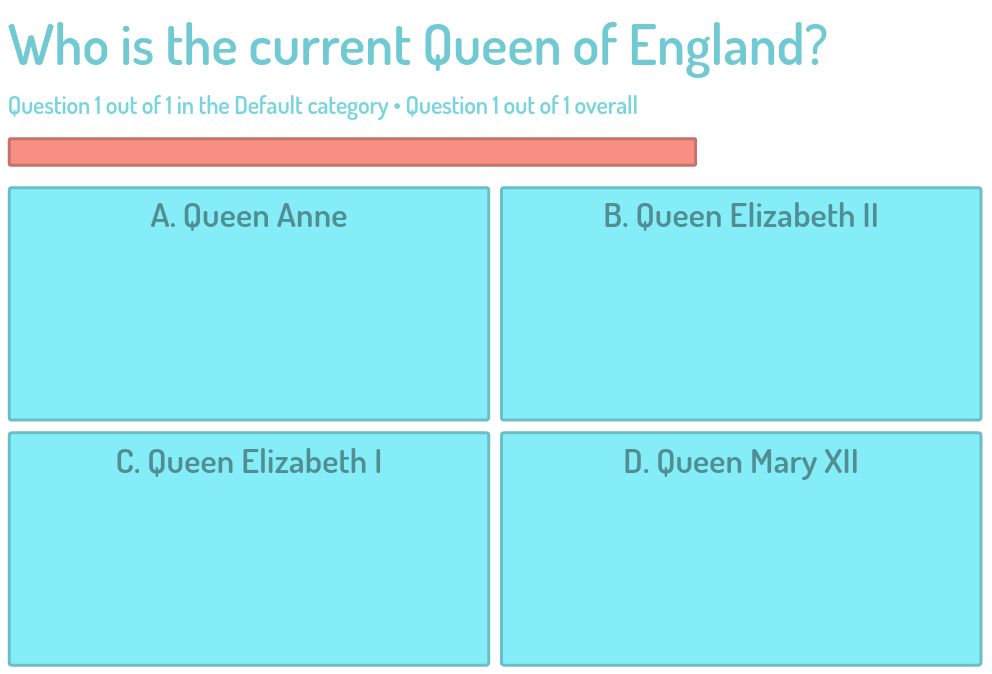
\includegraphics[scale=0.35]{user_guide/usage/play_quiz}
  \caption{The inteface shown when a quiz is in progress.}
\end{figure}

After a quiz has finished, all students will be shown a chart that lists the winner and how many house points each house got - this marks the end of the quiz.

\begin{figure}[h!]
  \centering
  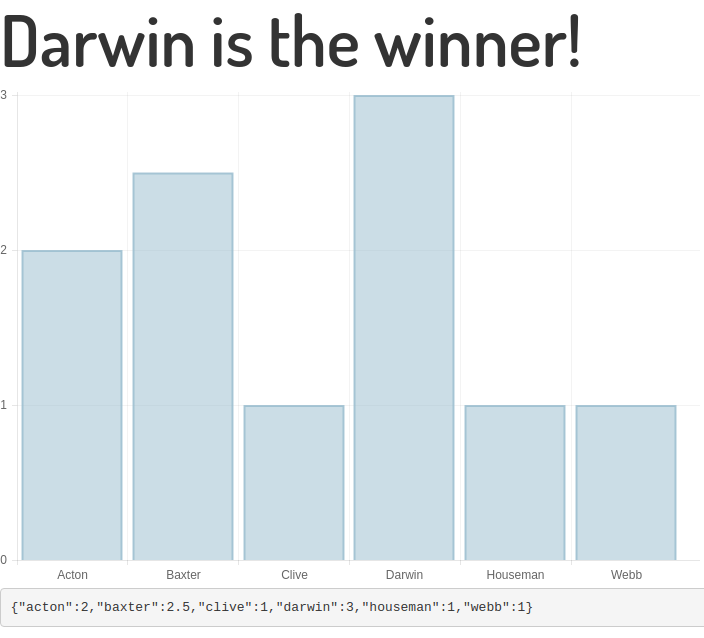
\includegraphics[scale=0.15]{user_guide/usage/results}
  \caption{The results chart shown at the end of the quiz.}
\end{figure}
% subsection playing_a_quiz (end)
% section usage (end)
